\documentclass[12pt, a4paper]{article}
\usepackage[utf8]{inputenc}
\usepackage{ 
    amsmath, amssymb, amsfonts, 
    amsthm, lipsum, 
    physics, mathtools, setspace,
    array, caption, float, subfig,
    tikz, tikz-3dplot
}

\usepackage[hmarginratio=1:1, margin=0.5in, includeheadfoot]{geometry}

\graphicspath{ {./res/} }
\usetikzlibrary{decorations.markings}
% \doublespacing 

\usepackage{xcolor}
% \pagecolor[rgb]{0.128,0.128,0.128}
% \color[rgb]{1,1,1}

\title{\vspace{-3cm}Applications of Quaternions in 3D Rotation}
\author{Martin Velikov}
\date{To what extent can quaternions supersede rotation matrices and Euler
    angles in representing 3D rotation?}

\begin{document}

\maketitle
\tableofcontents

\pagebreak

\section{Introduction}
In the modern day, digital entertainment industries aim to replicate and extend
the appearance of our 3D world for artistic effects. Extensive use of 3D
computer graphics is made in films through CGI (computer generated imagery), or
in video games through real-time rendering on the player's device. Every day,
scientists conduct simulation research in three dimensional spaces, i.e. in the
fields of aerodynamic modeling, astrophysics, weather modelling and
computational chemistry. In all of these use cases, there is a need for a
rigorous mathematical framework to represent and manipulate the 3D world. \\

\subsection{Three Dimensional Objects}
In the real world, matter is composed of atoms which move on a microscopic
level. Any interaction with objects results in the collective transformation of
these atoms, perceived by us as something moving. In the simulated world, it is
not practical to simulate the granular motion of the billions of atoms in a
single object, hence the need for simplification of the way objects are
represented. \\

The conventional approach to creating a three dimensional world is to split it
into intuitive chunks, called "3D models". For example, in a scene with a teapot
resting on a wooden table, it would make sense to split the teapot and the table
into separate 3D models, to perform calculations on each of them individually.
For example, one may wish to move just the teapot, without moving the table. \\

% In computer graphics, the shape of these objects is represented by a few
% properties.

\subsubsection{Vertices}
Every object can be represented with a set of three-dimensional points along its
surface (called "vertices") which define its shape. For maximum detail, vertices
are usually placed where the shape of the object changes most, like on the
object's edges or corners. Increasing the number of vertices increases the
detail of the 3D model's shape.

\subsubsection{Edges \& Faces}
Edges are three dimensional straight lines connecting %two or more
three vertices together, forming a "wireframe" of the object. Faces are filled
planes between three edges, in total connected to three vertices. In this way, an
object with a complex shape is approximated to a certain precision with a number
of faces proportional to the desired precision. \\

Using this method, nearly every three dimensional object one wants to represent
can be approximated with a finite number of vertices, edges and faces. \\

\begin{figure}[H]
    \centering
    \subfloat[Cube]{
        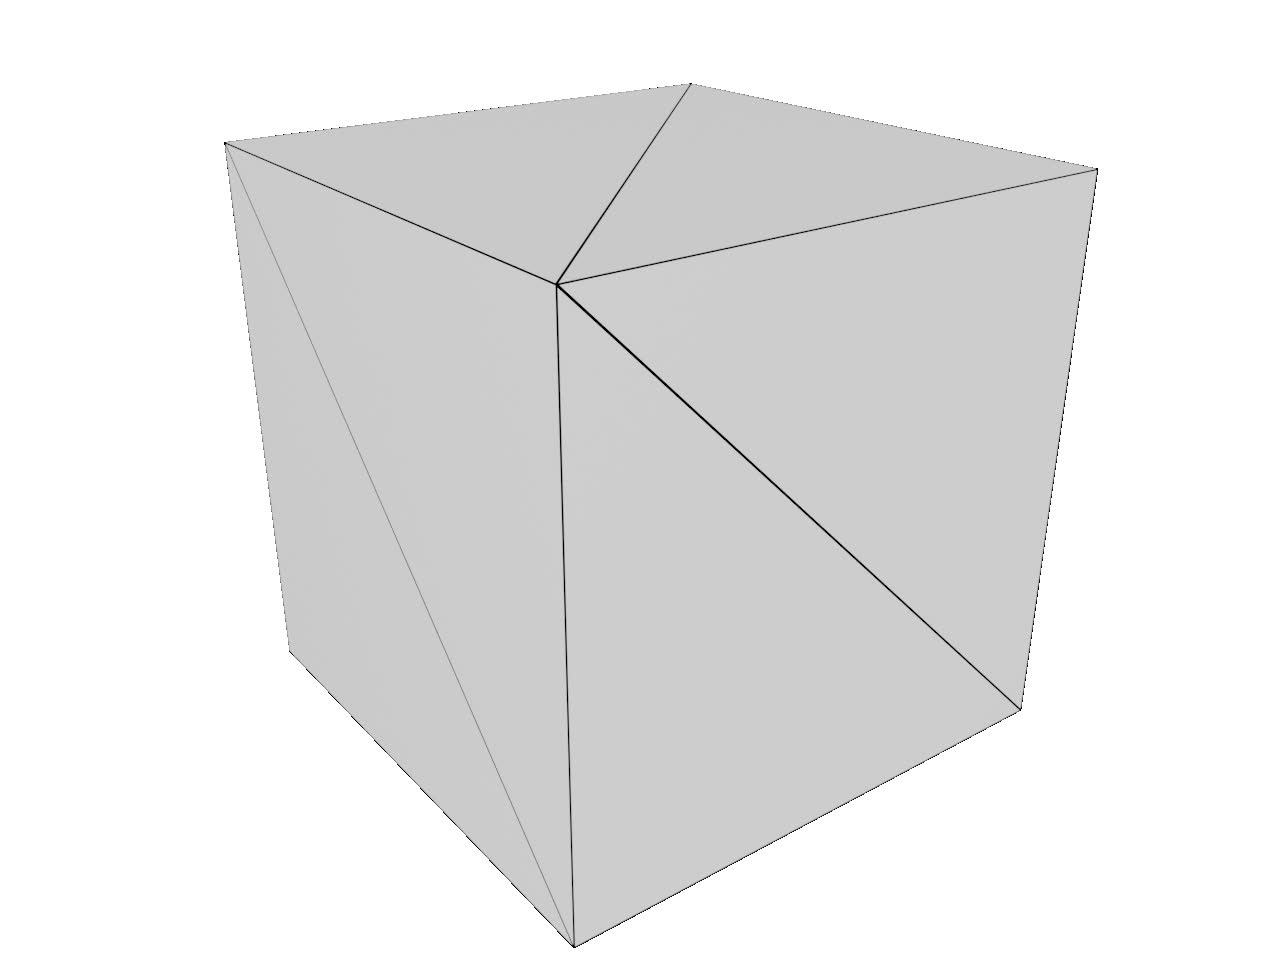
\includegraphics[width=5cm]{cube_wireframe.jpg}
    }
    \qquad
    \subfloat[Sphere]{
        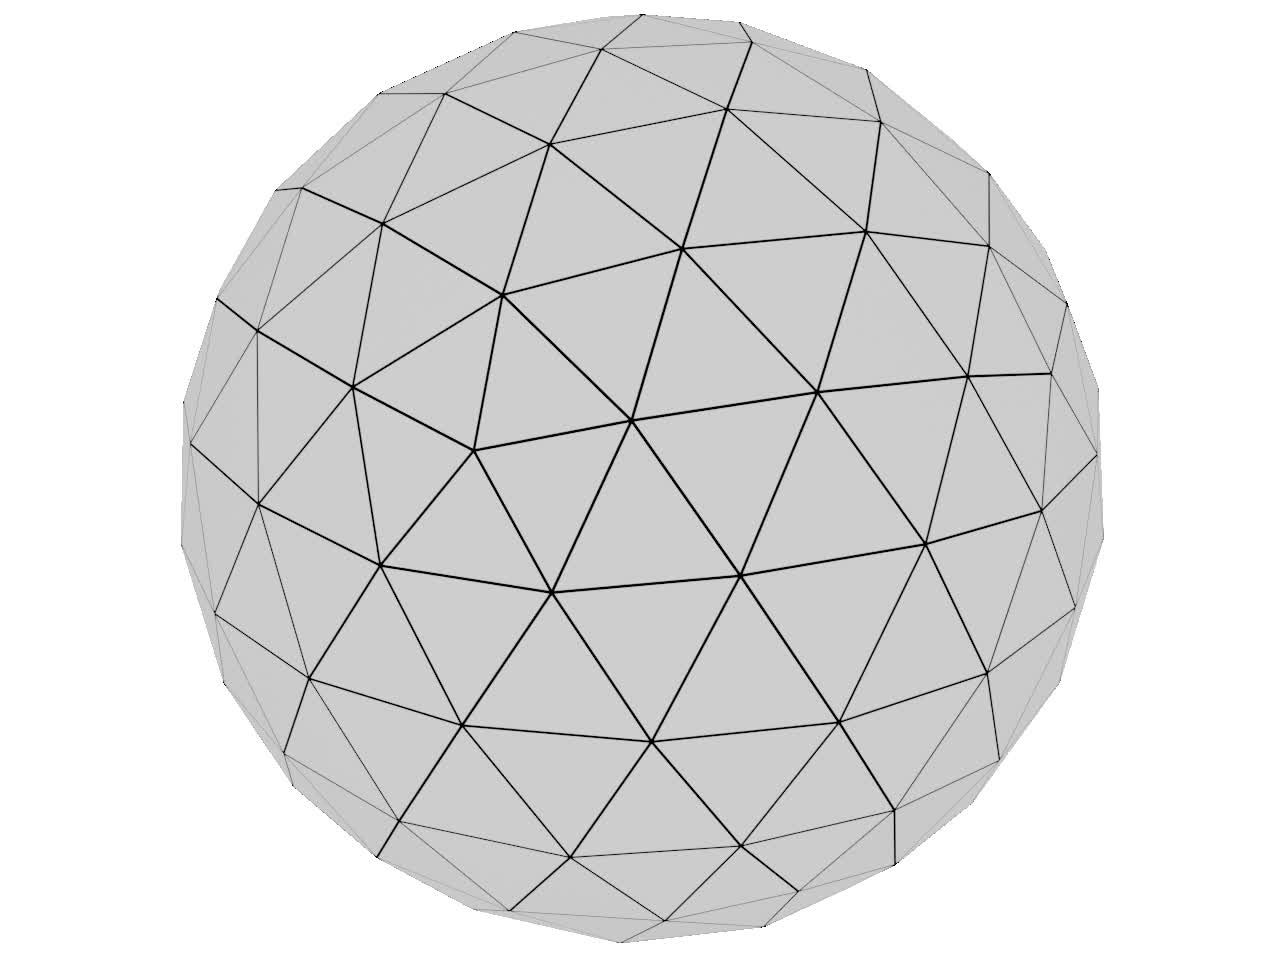
\includegraphics[width=5cm]{icosphere_wireframe.jpg}
    }
    \qquad
    \subfloat[Teapot]{
        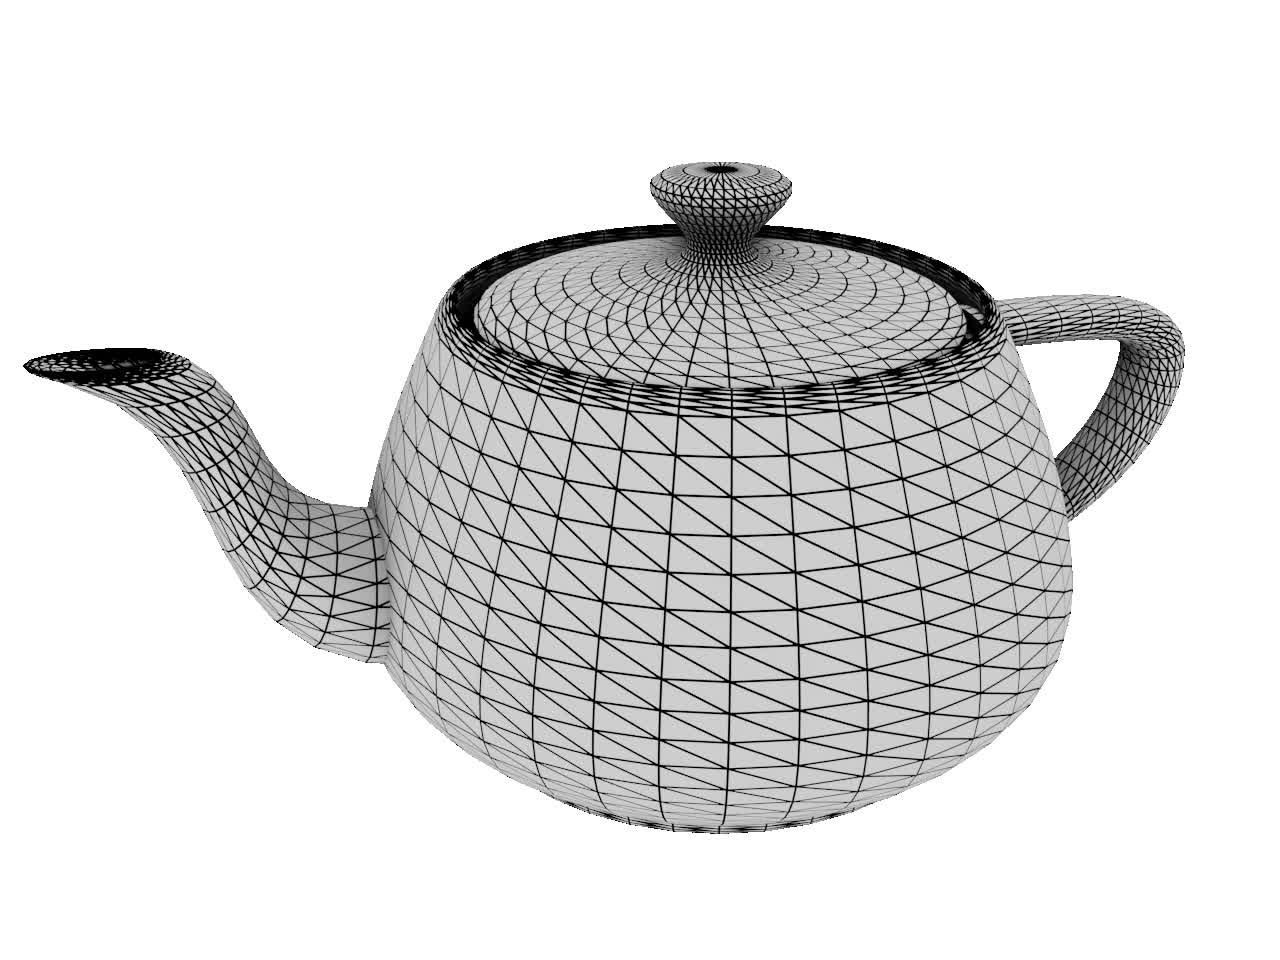
\includegraphics[width=5.75cm]{teapot_wireframe.jpg}
    }
    \caption{Wireframe view of various 3D objects}
    \label{teapot}
\end{figure}

% A face with three vertices is called a "triangle", and a face with
% four vertices is called a "quad". While triangles are ensured to be planar,
% quads are not, meaning that it is difficult to concretely define their normals.
% For this reason, quads are usually "triangulated" into two triangles. For any
% models in this investigation, we will assume that all faces are triangles.\\

\subsection{3D Transformations}
In the real world, objects are not static. They move, rotate and change shape
through time. In the simulated world, it is necessary to be able to perform
similar transformations on the 3D models. A valuable property of the
vertex-edge-face object representation is that transformations on a whole
object are a product of smaller transformations on its comprising vertices. \\

\subsubsection{Translation}
Translation is the simplest transformation, and is defined as the movement of an
object along a vector. For example, if an object is translated by the vector
$(1, 2, 3)$, it will move by 1 unit along the $x$ axis, 2 units along the $y$
axis and 3 units along the $z$ axis. In order to translate an object, one would
simply add the vector to the co-ordinates of each of its vertices. \\

\subsubsection{Scale}
Scaling is the dilation of an object by a factor along each of the three axes.
For example, if an object is scaled by a factor of 2 along the $x$ axis, it will
be twice as wide as before. In order to scale an object, one would simply
multiply the co-ordinates of each of its vertices by the scale factor. A uniform
scale refers to dilating an object by all three of the axes equally, which would
make the object bigger or smaller, but maintain its proportions. \\

\subsubsection{Rotation}
Rotation is one of the more complex transformations. It is defined as the
movement of an object's vertices in such a way so that the object appears to
rotate, while its shape remains unchanged. However, the concept of rotation
could be ambiguous in that it is not clear how exactly the object should rotate.
One could rotate the object around the origin, or around its center of mass, or
in fact around any arbitrary point of reference in 3D space. \\

Due to its complexity, there have been many different ways of defining and
implementing rotation in three dimensions by many different mathematicians such
as Leonard Euler, William Rowan Hamilton and Olinde Rodrigues. \\

Currently, there are three main methods of describing rotation in 3D space:
Euler angles, rotation matrices and quaternions. In this investigation, we will
compare and contrast these different rotational methods in order to draw
conclusions about the usefulness and applicability of quaternions in 3D computer
graphics and scientific simulations.

\section{Rotation Matrices}
\subsection{Object \& world axes}
Any object transformation can be represented by where its three axes "end up"
after the transformation. The direction of each axis is represented as a 3D
vector of norm one, which "points" in the desired direction. However, the
meaning of the "object's axes" is ambigous here. It is important to make the
distinction between the "world axes" which represent the axes of the surrounding
3D scene, and the "object axes", which describe it in its own space, as if it
were the only object in a scene. The useful property of this abstraction is that
the object axes do not necessary have to be oriented the same as the world axes,
and this can be leveraged for transformation. \\

The three object X,Y,Z axes can be represented by the vectors
$\vec{x}$, $\vec{y}$, $\vec{z}$: \\

\begin{align*}
    \vec{x} = \begin{bmatrix} 1 \\ 0 \\ 0 \end{bmatrix}
    \quad
    \vec{y} = \begin{bmatrix} 0 \\ 1 \\ 0 \end{bmatrix}
    \quad
    \vec{z} = \begin{bmatrix} 0 \\ 0 \\ 1 \end{bmatrix}
\end{align*} \\

This orientation of the axes is called the "identity". It describes a space
where all three axes are perpendicular, and are aligned with the world axes.

\subsection{Rotating points}
\label{rotating_points}

Whenever a point $\vec{p}$ has to be rotated, its X,Y and Z components ($p_x$,
$p_y$ and $p_z$ respectively) can be multiplied by their respective object axis.

\begin{align*}
    \vec{a} = \vec{x}p_x
    \quad
    \vec{b} = \vec{y}p_y
    \quad
    \vec{c} = \vec{z}p_z
    \quad
\end{align*}

The resulting vectors are then added together for the final position of
the transformed point $\vec{r}$.

\begin{align*}
    \vec{r} = \vec{a} + \vec{b} + \vec{c}
\end{align*}

\subsubsection{3$\times$3 Matrix form}
The process of transforming $\vec{p} \rightarrow \vec{r}$ is highly reminiscent of matrix
multiplication. It is useful to represent $\vec{x}$, $\vec{y}$, $\vec{z}$ as a
single 3$\times$3 matrix of their components $M$ of the form

\begin{align*}
    M = \begin{bmatrix}
            {\vec{x}}_x & {\vec{y}}_x & {\vec{z}}_x \\
            {\vec{x}}_y & {\vec{y}}_y & {\vec{z}}_y \\
            {\vec{x}}_z & {\vec{y}}_z & {\vec{z}}_z
        \end{bmatrix}
\end{align*}

The transformation of $\vec{p}$ to $\vec{r}$ can then be described by $M\vec{p}$
because of the properties of matrix multiplication, in that

\begin{align*}
    M\vec{p} = \vec{M_1}p_x + \vec{M_2}p_y + \vec{M_3}p_z
    \quad \text{where $M_n$ represents the $n$th column of $M$.}
\end{align*}

Since the columns $\vec{M_1}$, $\vec{M_2}$, $\vec{M_3}$ correspond to the object
axes X, Y and Z respectively, this is equrivalent to the rotation equation shown
in Section \ref{rotating_points}. \\

In this form, the identity axes are represented by the matrix $I = \begin{bmatrix}
    1 & 0 & 0 \\
    0 & 1 & 0 \\
    0 & 0 & 1
\end{bmatrix}$.

% \begin{align*}
    
% \end{align*}

\subsection{Construction from Euler angles}

\subsubsection{Concept}
In real life, it is practical to represent rotations with easily measurable
metrics, like angles. Aircraft and watercraft make extensive use of yaw, pitch
and roll angles in instrumentation to aid their pilots in judging the orientation
of the craft. \\

Euler angles are based around this concept. A set of Euler angles is a 3D vector
containing the yaw, pitch and roll of an object from a reference frame. In the
example of aircraft, the reference frame is usually the surface of the Earth. In
space, it is usually a prominent constellation or celestial object.

It is possible to construct rotation matrices for a rotation of $\theta$ around
each axis.

\subsubsection{Deriving rotation matrices for each angle}
Consider rotating the identity axes by $\theta$ around the X axis. Let the
rotation matrix that describes this transformation be $R_x$. \\

% TODO: insert figure

\begin{figure}[H]
    \centering
    \tdplotsetmaincoords{70}{50}
    \begin{tikzpicture}[x=0.5cm,y=0.5cm,z=0.3cm,>=stealth,tdplot_main_coords]
        \coordinate (X) at (5,0,0);
        \coordinate (Y) at (0,3,0);
        \coordinate (Z) at (0,0,3);

        \draw[->, red] (0,0,0) -- (X) node[right] {$x, \, R_{x_x}(\theta)$};
        \draw[->, blue] (0,0,0) -- (Y) node[right] {$y$};
        \draw[->, black!60!green] (0,0,0) -- (Z) node[above] {$z$};

        \begin{scope}[canvas is zy plane at x=0]
            \draw[dashed, darkgray] (0,0) circle (3);
            \draw[->, blue, dashed] (0,0) -- ({sin(20)*3}, {cos(20)*3}) node[right] {$R_{x_y}(\theta)$};
            \draw[->, black!60!green, dashed] (0,0) -- ({sin(110)*3}, {cos(110)*3}) node[left] {$R_{x_z}(\theta)$};

            \draw[black!30!blue] (0.26,1.5) node {$\theta$};
            \draw[black!80!green] (1.5,-0.26) node {$\theta$};
        \end{scope}

    \end{tikzpicture}
    \caption{Rotation around the X-axis by angle $\theta$. $R_{x_x}, R_{x_y}$
        and $R_{x_z}$ represent the object axes after the transformation by
        $R_x(\theta)$ where $x \to R_{x_x}, y \to R_{x_y}$ and $z \to R_{x_z}$}
    \label{rot_x}
\end{figure}

From Figure \ref{rot_x} it becomes apparent that points that lie along the identity X-axis do
not move at all. Hence, for the first column $R_{x_x}$ representing the object
X-axis post-transform,

\begin{align*}
    R_{x_x}(\theta) = x = \begin{bmatrix} 1 \\
                              0 \\ 0\end{bmatrix}
\end{align*}

Points that lie along the Y axis get transformed against a circle of radius one
along the YZ plane, meaning  its coordinates are described by the trigonometric
functions sine and cosine. Hence,

\begin{align*}
    R_{x_y}(\theta) = \begin{bmatrix} 0 \\ \cos\theta \\ \sin\theta
                      \end{bmatrix}
\end{align*}

The Z-axis corresponds to the circle's Y-axis on a cartesian plane (along the 3D
YZ plane), so it is as if the Z-axis was rotated by a right angle, then by
$\theta$. Hence,

\begin{align*}
    R_{x_z}(\theta)
    = \begin{bmatrix}
          0                            \\
          \cos(\theta + \frac{\pi}{2}) \\
          \sin(\theta + \frac{\pi}{2})
      \end{bmatrix}
    = \begin{bmatrix}
          0           \\
          -\sin\theta \\
          \cos\theta
      \end{bmatrix}
\end{align*}.

Finally, combining $R_{x_x}, R_{x_y}$ and $R_{x_z}$,

\begin{align*}
    R_x(\theta)
    = \begin{bmatrix}
          1 & 0          & 0           \\
          0 & \cos\theta & -\sin\theta \\
          0 & \sin\theta & \cos\theta
      \end{bmatrix}
\end{align*}

A very similar process can be followed for the rotation matrices by the Y
($R_y$) and Z ($R_z$) axes, so it has been omitted for brevity. The only thing
that changes in the process is that the plane of the circle follows the two axes
perpendicular to the rotation axis.

\begin{align*}
    R_y(\theta) = \begin{bmatrix}
                      \cos \theta  & 0 & \sin \theta \\
                      0            & 1 & 0           \\
                      -\sin \theta & 0 & \cos \theta
                  \end{bmatrix}
    \quad
    R_z(\theta) = \begin{bmatrix}
                      \cos \theta & -\sin \theta & 0 \\
                      \sin \theta & \cos \theta  & 0 \\
                      0           & 0            & 1
                  \end{bmatrix}
\end{align*}

\subsubsection{Multiplication}

For the Euler angles $\alpha$, $\beta$ and $\gamma$ representing yaw, pitch and
roll respectively, it is now possible to compute a general rotation matrix by
first constructing each individual matrix, then multiplying them.

\begin{align*} \\
    R(\alpha, \beta, \gamma) & = R_z(\gamma) R_y(\beta) R_x(\alpha)                                                                                                \\
                             & = \begin{bmatrix}
                                     \cos \gamma & -\sin \gamma & 0 \\
                                     \sin \gamma & \cos \gamma  & 0 \\
                                     0           & 0            & 1 \\
                                 \end{bmatrix}
    \begin{bmatrix}
        \cos \beta  & 0 & \sin \beta \\
        0           & 1 & 0          \\
        -\sin \beta & 0 & \cos \beta \\
    \end{bmatrix}
    \begin{bmatrix}
        1 & 0           & 0            \\
        0 & \cos \alpha & -\sin \alpha \\
        0 & \sin \alpha & \cos \alpha  \\
    \end{bmatrix}                                                                                                                                 \\
                             & = \begin{bmatrix}
                                     \cos\beta\cos\gamma & \sin\alpha\sin\beta\cos\gamma - \cos\alpha\sin\gamma & \cos\alpha\sin\beta\cos\gamma + \sin\alpha\sin\gamma \\
                                     \cos\beta\sin\gamma & \sin\alpha\sin\beta\sin\gamma + \cos\alpha\cos\gamma & \cos\alpha\sin\beta\sin\gamma - \sin\alpha\cos\gamma \\
                                     -\sin\beta          & \sin\alpha\cos\beta                                  & \cos\alpha\cos\beta                                  \\
                                 \end{bmatrix}
\end{align*} \\

As matrix multiplication does not commute, it is not always the case that
rotating by an axis A, then rotating by B would be the same as rotating first by
axis B, then by A. Hence, it is important to note that the order of
multiplication of $R_z$, $R_y$ and $R_x$ produces a unique final rotation. For
the rest of the investigation, the $z \to y \to x$ rotation order seen above
will be used. This is alternatively called the ZYX Tait-Bryan order.

\subsection{The gimball lock problem}
There is one large problem with constructing rotation matrices from Euler
angles. Suppose you rotated an object with the Euler angles
$\alpha$, $\beta$ and $\gamma$, where $\beta=\frac{\pi}{2}$

\begin{align*} \\
    R(\alpha, \frac{\pi}{2}, \gamma)
     & = \begin{bmatrix}
             \cos\frac{\pi}{2}\cos\gamma & \sin\alpha\sin\frac{\pi}{2}\cos\gamma - \cos\alpha\sin\gamma & \cos\alpha\sin\frac{\pi}{2}\cos\gamma + \sin\alpha\sin\gamma \\
             \cos\frac{\pi}{2}\sin\gamma & \sin\alpha\sin\frac{\pi}{2}\sin\gamma + \cos\alpha\cos\gamma & \cos\alpha\sin\frac{\pi}{2}\sin\gamma - \sin\alpha\cos\gamma \\
             -\sin\frac{\pi}{2}          & \sin\alpha\cos\frac{\pi}{2}                                  & \cos\alpha\cos\frac{\pi}{2}                                  \\
         \end{bmatrix}
    \\
     & = \begin{bmatrix}
             0  & \sin\alpha\cos\gamma - \cos\alpha\sin\gamma & \cos\alpha\cos\gamma + \sin\alpha\sin\gamma \\
             0  & \sin\alpha\sin\gamma + \cos\alpha\cos\gamma & \cos\alpha\sin\gamma - \sin\alpha\cos\gamma \\
             -1 & 0                                           & 0                                           \\
         \end{bmatrix}
    \\
     & = \begin{bmatrix}
             0  & \sin(\alpha - \gamma) & \cos(\alpha - \gamma)  \\
             0  & \cos(\alpha - \gamma) & -\sin(\alpha - \gamma) \\
             -1 & 0                     & 0                      \\
         \end{bmatrix}
\end{align*} \\

Notice how in the above matrix, changing the value of both $\alpha$ and $\gamma$
would result in a rotation around the world Z-axis as 

\begin{align*}
    R_1 = \begin{bmatrix} 0  \\
        0  \\
        -1 \\
    \end{bmatrix}
\end{align*} \\

Hence, one degree of freedom is lost here - it is not possible to rotate the
object by any other axis than the Z world axis, by changing either $\alpha$ or
$\gamma$. This problem specifically occurs whenever you rotate around an axis by
90 degrees, and "align" it with another. \\

This fundamental flaw with Euler angles demonstrates how despite their
simplicity and intuitiveness, they are not always the best choice for
representing rotations. \\

In the Apollo 11 mission, (talk about gimball lock)

\subsection{The spherical linear interpolation problem}

\section{Quaternions}
\subsection{Axis-angle}
Another interesting way to represent the rotation of an object 

\subsection{Standard Form}
Quaternions, like complex numbers, are defined with "real" and "imaginary"
parts, and are essentially an extension of the complex numbers to four
dimensions. The set of all quaternions is known as $\mathbb{H}$, named after the
last initial of the Irish mathematician William Rowan Hamilton. Algebraically, a
quaternion $q$ can be defined in terms of the coefficients of its terms:

\begin{align*}
    q = a + bi + cj + dk \quad a, b, c, d \in \mathbb{R}
\end{align*}

$i$, $j$ and $k$, called "basic quaternions", do not have an explicit definition
of their value but are rather defined expressly in terms of the way they
interact with each other in that they must satisfy the equality

\begin{align*}
    i^2 = j^2 = k^2 = ijk = -1
\end{align*}

\subsection{Basic Quaternions}

\subsubsection{Multiplying by Real Numbers}
For any $n \in \mathbb{R}$, it is defined that $in = ni$, $jn = nj$ and $kn =
    nk$. Hence, for any $q \in \mathbb{H}$, $qn = nq$. Quaternion multiplication by
real numbers does, in fact, commute.

\subsubsection{Multiplication by other basic quaternions}
Hamilton's quaternion definition can then be used to derive the multiplicative
interactions between $i$, $j$ and $k$:

% ij & jk
\begin{align*}
     &
    \begin{aligned}
        ijk    & = k^2   \\
        ijk^2  & = k^2k  \\
        ij(-1) & = (-1)k \\
        ij     & = k
    \end{aligned}
     &
    \begin{aligned}
        ijk    & = i^2         \\
        i^2 jk & = i \cdot i^2 \\
        (-1)jk & = i(-1)       \\
        jk     & = i
    \end{aligned}
\end{align*}

% kj and ji
\begin{align*}
     &
    \begin{aligned}
        i  & = jk   \\
        ji & = j^2k \\
        ji & = -k
    \end{aligned}
     &
    \begin{aligned}
        k  & = ij   \\
        kj & = ij^2 \\
        kj & = -i
    \end{aligned}
\end{align*}

% ki & ik
\begin{align*}
     &
    \begin{aligned}
        ij     & = k     \\
        kij    & = k^2   \\
        kij^2  & = k^2j  \\
        ki(-1) & = (-1)j \\
        ki     & = j
    \end{aligned}
     &
    \begin{aligned}
        k  & = ij   \\
        ik & = i^2j \\
        ik & = -j
    \end{aligned}
\end{align*}

An important concept becomes apparent from the above calculations - quaternion
multiplication by other quaternions is not commutative, that is, it can be the
case that $q_1q_2 \neq q_2q_1$ where $ q_1,q_2 \in \mathbb{H}$. For example, it
is seen above that while $ij = k$, $ji = -k$. \\

The multiplication table of basic quaternions is hence formed:

\begin{center}
    \doublespacing
    \begin{tabular}{ | c | c | c | c | }
        \hline
        $\times$ & $i$  & $j$  & $k$  \\
        \hline
        $i$      & $-1$ & $-k$ & $j$  \\
        \hline
        $j$      & $k$  & $-1$ & $-i$ \\
        \hline
        $k$      & $-j$ & $i$  & $-1$ \\
        \hline
    \end{tabular}
    \captionof{table}{Basic quaternion noncommutative multiplication table}\label{sophisticatedtable}
\end{center}

\subsubsection{Associativity}
Quaternion multiplication is associative in that $(q_1 q_2) q_3 = q_1 (q_2 q_3)$
where $q_1,q_2,q_3 \in \mathbb{H}$.
The same property applies for addition, $(q_1 + q_2) + q_3 = q_1 + (q_2 + q_3)$
where $q_1,q_2,q_3 \in \mathbb{H}$.

This associativity allows for application of useful algebraic
techniques like the distributive law.

\subsection{Quaternion Operations}
\subsubsection{Multiplication of non-basic quaternions}
Let $q_1 = a_1 + b_1i + c_1j + d_1k$ and $q_2 = a_2 + b_2i + c_2j + d_2k$ where
$a_1, b_1, c_1, d_1, a_2, b_2, c_2, d_2 \in \mathbb{R}$. The multiplication
$q_1q_2$ can be computed using the distrivutive law.

\begin{align*}
    q_1q_2 & = (a_1 + b_1i + c_1j + d_1k)(a_2 + b_2i + c_2j + d_2k)    \\
           & = a_1a_2 + a_1b_2i + a_1c_2j + a_1d_2k                    \\
           & + b_1a_2i + b_1b_2i^2 + b_1c_2ij + b_1d_2ik               \\
           & + c_1a_2j + c_1b_2ji + c_1c_2j^2 + c_1d_2jk               \\
           & + d_1a_2k + d_1b_2ki + d_1c_2kj + d_1d_2k^2               \\
           & \text{Applying the basic quaternion rules then}           \\
           & \text{factoring out the real part and $i$, $j$, and $k$,} \\
           & = a_1a_2 - b_1b_2 - c_1c_2 - d_1d_2                       \\
           & + (a_1b_2 + b_1a_2 + c_1d_2 - d_1c_2)i                    \\
           & + (a_1c_2 - b_1d_2 + c_1a_2 + d_1b_2)j                    \\
           & + (a_1d_2 + b_1c_2 - c_1b_2 + d_1a_2)k
\end{align*}

\subsubsection{Conjugation}
For any quaternion $q = a + bi + cj + dk \quad a, b, c, d \in \mathbb{R}$, its
conjugate $q^*$ is defined as $q^* = a - bi - cj - dk$. \\

\subsubsection{Multiplication by Conjugate}
Suppose one was to multiply a quaternion $q$ by its conjugate $q^*$,
\begin{align*}
    qq^* & = (a + bi + cj + dk)(a - bi - cj - dk)            \\
         & = a^2 - abi - acj - adk                           \\
         & + bia - (bi)^2 - bicj - bidk                      \\
         & + cja - cjbi - (cj)^2 - cjdk                      \\
         & + dka - dkbi - dkcj - (dk)^2                      \\
         & \text{Reordering real coefficients and expanding} \\
         & = a^2 - abi - acj - adk                           \\
         & + abi - b^2i^2 - bcij - bdik                      \\
         & + acj - bcji - c^2j^2 - cdjk                      \\
         & + adk - bdki - cdkj - d^2k^2                      \\
         & \text{Applying basic quaternion rules}            \\
         & = a^2 - abi - acj - adk                           \\
         & + abi + b^2 - bck + bdj                           \\
         & + acj + bck + c^2 - cdi                           \\
         & + adk - bdj + cdi + d^2                           \\
    \\
         & a, b, c, d \in \mathbb{R}                         \\
         & \therefore a^2 + b^2 + c^2 + d^2 \in \mathbb{R}
\end{align*}

Hence, if you multiply a quaternion by its conjugate, the result will always be
a real number and equal to the sum of the squares of its coefficients.

% https://www.quora.com/How-do-I-find-the-inverse-of-a-quaternion

\subsubsection{Inverse}
The inverse $q^{-1}$ of a quaternion $q = a + bi + cj + dk$ exists such that $qq^{-1} = 1$,
effectively "undoing" any multiplication caused by $q$. The inverse of a
quaternion can be computed using the previosuly established rules.

\begin{align*}
     & qq^{-1} = 1 \Rightarrow q^{-1} = \frac{1}{q}         \\
     & \frac{1}{q} \cdot \frac{q^*}{q^*} = \frac{q^*}{qq^*}
    = \frac{q^*}{a^2 + b^2 + c^2 + d^2}
\end{align*}

\subsection{Proof that $qpq^{-1}$ returns a pure quaternion}

Whenever a pure quaternion is multiplied by a rotation quaternion, the
transformation inevitably distorts it into the fourth dimension.

% https://math.stackexchange.com/questions/1354627/why-is-it-so-that-a-unit-quaternion-t-can-be-written-as-t-cos-thetau-sine
% cos^2 \theta + sin^2 \theta = 1

\begin{align*}
    qp     & = (a_qa_p - b_qb_p - c_qc_p - d_qd_p)                \\
           & + (a_qb_p + b_qa_p + c_qd_p - d_qc_p)i               \\
           & + (a_qc_p - b_qd_p + c_qa_p + d_qb_p)j               \\
           & + (a_qd_p + b_qc_p - c_qb_p + d_qa_p)k               \\
           & \text{Let:\space}                                    \\
    a_{qp} & = a_qa_p - b_qb_p - c_qc_p - d_qd_p,                 \\
    b_{qp} & = a_qb_p + b_qa_p + c_qd_p - d_qc_p,                 \\
    c_{qp} & = a_qc_p - b_qd_p + c_qa_p + d_qb_p,                 \\
    d_{qp} & = a_qd_p + b_qc_p - c_qb_p + d_qa_p                  \\
    \\
           & \text{As q is of norm one, } q^{-1} = q^*            \\
           & \therefore qpq^{-1} = qpq^*                          \\
           & = a_{qp}a_q + b_{qp}b_q + c_{qp}c_q + d_{qp}d_q      \\
           & + (- a_{qp}b_q + b_{qp}a_q - c_{qp}d_q + d_{qp}c_q)i \\
           & + (- a_{qp}c_q + b_{qp}d_q + c_{qp}a_q - d_{qp}b_q)j \\
           & + (- a_{qp}d_q - b_{qp}c_q + c_{qp}b_q + d_{qp}a_q)k \\
\end{align*}

In order for $qpq^*$ to be pure, its real part must be equal to zero. \\
Let $a_{qpq^*}$ be the real part of $qpq^*$.

\begin{align*}
    a_{qpq^*} & = a_{qp}a_q + b_{qp}b_q + c_{qp}c_q + d_{qp}d_q                            \\
              & = a_q(a_qa_p - b_qb_p - c_qc_p - d_qd_p)                                   \\
              & + b_q(a_qb_p + b_qa_p + c_qd_p - d_qc_p)                                   \\
              & + c_q(a_qc_p - b_qd_p + c_qa_p + d_qb_p)                                   \\
              & + d_q(a_qd_p + b_qc_p - c_qb_p + d_qa_p)                                   \\
              & =a_q^2a_p - a_qb_qb_p - a_qc_qc_p - a_qd_qd_p                              \\
              & + b_qa_qb_p + b_q^2a_p + b_qc_qd_p - b_qd_qc_p                             \\
              & + c_qa_qc_p - c_qb_qd_p + c_q^2a_p + c_qd_qb_p                             \\
              & + d_qa_qd_p + d_qb_qc_p - d_qc_qb_p + d_q^2a_p                             \\
              & = a_q^2a_p + b_q^2a_p + c_q^2a_p + d_q^2a_p                                \\
              & = a_p(a_q^2 + b_q^2 + c_q^2 + d_q^2)                                       \\
              & = a_p = 0                                                                  \\
              & \therefore qpq^{-1} \text{ is pure for } ||q||^2 = 1, \mathfrak{Re}(p) = 0
\end{align*}

\end{document}

% https://apollo11space.com/apollo-and-gimbal-lock/

% hello 